\documentclass[12pt]{article}
\usepackage[a4paper]{geometry}
\usepackage[utf8]{inputenc}
\usepackage[T1]{fontenc}
\usepackage[english]{babel}
\usepackage{mathtools}
\usepackage{amsfonts}
\usepackage{amsmath}
\usepackage{hyperref}
\usepackage{subcaption}
\usepackage[dvipsnames]{xcolor}
\usepackage[toc,page]{appendix}
\usepackage{multicol}
\usepackage{inconsolata}
\usepackage{listings}
\lstset{basicstyle=\ttfamily\footnotesize}
\hypersetup{
    colorlinks=true,
    linkcolor=RoyalPurple,   
    urlcolor=RoyalPurple
}

\title{Oscilloscope vector graphics on a \mbox{Telequipment D54} using an \mbox{Arduino MKR Vidor 4000}}
\author{Teodora Osiac \and Ioan Dragomir}
\date{January 2021}

\begin{document}

\makeatletter
\renewcommand{\and}{\quad}
\begin{titlepage}
	\vspace*{\fill}
	\centering

	\makeatletter
	\centering{\LARGE\bfseries \@title \par} \vspace{1.5cm}

	
\includegraphics[height=1.5in]{images/tucn-logo.jpg}\par

	\vspace{1.5cm}
	{\Large\@author \par}\vspace{0.45cm}

	{\large supervised by\par
	Prof. Dr. Radu Fechete}

	\vspace*{\fill}
	{\large \@date\par}
\end{titlepage}
\makeatother

\begin{abstract}
\noindent Displaying line art on an oscilloscope in XY mode is a common entry level electronics project, which is much beloved by hobbyists worldwide, both for the ease of obtaining minimally functional graphics, as well as the plentiful challenging enhancements it often invites. We aim to display both static vector art, as well as animations at a perceptually smooth refresh rate, while providing a resolution finer than the trace width (cca. 0.5mm), and covering as much of the 10x6cm screen of the Telequipment D54 as possible. We develop a hardware and software stack that enables programming an Arduino MKR Vidor 4000 with static vector art, as well as streaming live animations at 192000 points/second via USB.

\end{abstract}

\tableofcontents

\newpage

\section{Introduction}

In the 1960s and 1970s, CRT vector displays were an important advancement in computer graphics technology, a natural follow-up to the oscilloscope displays developed since the early 1900s. As opposed to raster CRT displays (as found in TV sets) which have a fixed beam path and modulate its intensity, vector displays have a mostly fixed electron beam intensity and control its position, tracing arbitrary monochrome paths on the screen. Vector displays were used with early CAD software (Ivan Sutherland's Sketchpad, 1963) and fighter aircraft HUDs, but notably also entered the home market and gained some popularity with the advent of vector arcade games in the 1980s. Games such as Asteroids and the Vectrex console have been since remembered for their distinct graphics style, and so displaying vector graphics on a CRT screen, usually that of an oscilloscope in XY mode, remains a common hobbyist project to this day.

Controlling a vector display consists in coordinating two waveforms -- one for the horizontal beam deflection and one for the vertical beam deflection, to position the electron beam arbitrarily on the screen. Due to persistence of vision and the CRT phosphor's slow decay, the fast beam motion looks like streaks of light on the screen. Using this mechanism, various line graphics can be displayed.

We aim to develop an easily programmable system for processing vector graphics on a computer, transmitting the data to an Arduino, and generating the corresponding signals on the device. 

\newpage
\begin{figure}[h]
\centering

\includegraphics[width=0.85\textwidth]{images/demo-tucn.png}
\caption{Full display of the TUCN logo}
\label{fig:tucn-full}
\end{figure}
\section{Static signal generation}

To confirm the feasibility of the project, we start with a rudimentary software stack that enables programming an Arduino with a fixed, two-channel waveform corresponding to the X and Y coordinates of a point walking along a given path. The software consists of some javascript code that converts the first SVG <path> of the current document into a C header file containing a list of points (\autoref{appendix:svg2header}) and some Arduino code that iterates through the generated points and outputs each coordinate pair to the suitable ports (\autoref{appendix:staticvector}). At the hardware level, we require two DACs of sufficient resolution and sample rate, which motivates our choice of the Arduino MKR Vidor 4000, since it has a builtin 10-bit DAC, meaning we only have to implement a single DAC externally.

One of the requirements for a pleasant appearance is that we have control over the position of the beam in increments smaller than half the width of the beam itself. (\autoref{fig:low-resolution}) By some crude measurements, our device's beam is approximately 0.5 in diameter. To span 6cm vertically in increments less than 0.25mm, we require 240 distinct voltage levels, and thus at least 8 bits resolution for the vertical channel. Similarly, the horizontal channel requires at least \( \log_2{10\text{cm}/0.25\text{mm}} \approx 8.6 \) bits. Therefore we chose to use the built-in 10-bit DAC for the horizontal channel and to build an external 8-bit DAC for the vertical channel.

% http://falstad.com/circuit/circuitjs.html?ctz=CQAgjCAMB0l3BWcMBMcUHYMGZIA4UA2ATmIxAUgpABZsAoAJxGxRGMJbbGLarXhMu4Xu048+yQcw4juhKhKhS4Q2evGj+8SELAKx4A0u3SQAWlZzhJlbuaW2sx9dOqHspS9tgdQ8xoWnlogAu4W+oqiAZqSvmbmkYaJxiFh9hYoKDTWKVFxfg5ZOc7FrqGFmXh4uWU+leYo1clNNbbp-tgI3NGt5R0A5hZdPWyW3aHZyroA7kb5oQixUPQAHsOEENHY+uxIOVMAMgDKAEJrIiWc2ZyktKE5ALJn9Gjkjc2lzXhUOQAKAEsAHYAHQAzoRXpB3mVSlMfvdAaCwRgoe8ks4kgj-sDwXg0UFbpwYiBsSAkeDiASXM4rGSKWDfASrLI6b9ybjGWACYFZPTOWAUASMeIDPzkQwAPKLZaYUbTegAeweIEIOV+kDuMB0GEIKGI2GINAQOxQSG18DIhCWZuUbCmDCAA
\begin{figure}[h]
\centering
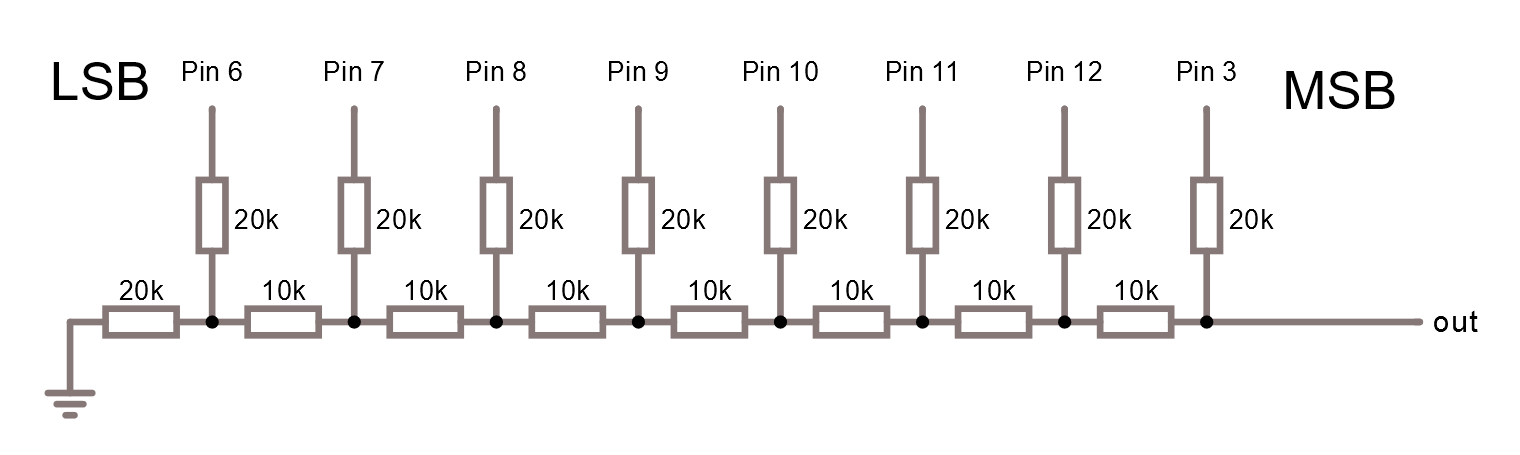
\includegraphics[width=0.99\textwidth]{images/r2r-circuit.png}
\caption{R-2R resistor ladder circuit for generating the vertical deflection signal}
\end{figure}

DAC design choice is a significant factor in both circuit complexity, cost, and the quality of the resulting graphics. We chose an R-2R ladder design for its relative simplicity, in spite of the expected DAC glitches (\autoref{fig:vertical-dac-glitches}) that appear when passing between points at a large Hamming distance but small Euclidean distance. (i.e., at coordinates at 1/2, 1/4, 3/4, etc. vertically along the screen)

To counteract such glitches, we ought to set all the output pins to their correct states at the same time, instead of setting each bit of the output sequentially. The Arduino standard library provides direct access to the PORTA register of the SAMD21 board, whose value is a bitmap of the digital values of 32 input or output pins. We use the Arduino pins 6, 7, 8, 9, 10, 11, 12, 3 (LSB to MSB) to control the resistor ladder, and these correspond to bits 20, 21, 16, 17, 19, 8, 9, 11 of the PORTA register. We apply the following bitwise permutation to obtain a value for the PORTA register given a desired 8 bit DAC output "Y", and assign all the bits at once:

\begin{lstlisting}
PORT->Group[PORTA].OUT.reg = ((Y & 0b11) << 20) |     // PA20, PA21
                             ((Y & 0b1100) << 14) |   // PA16, PA17
                             ((Y & 0b10000) << 15) |  // PA19
                             ((Y & 0b1100000) << 3) | // PA8, PA9
                             ((Y & 0b10000000) << 4); // PA11         
\end{lstlisting}
\noindent By doing so, the delay between the different pins being set to the correct value is far below noticeable, thus mostly solving the issue of DAC glitches. For improved performace, we precompute a lookup table for the 256 possible bit patterns, reducing the time to output an analog value from 23 instructions down to 5, (\autoref{appendix:lutoptimisation}) with a memory cost of 1KB.

Regardless of DAC design, an issue arises whereby signal bandwidth limitations (mostly justified by parasitic capacitance) in both the DAC, the scope probes, and the oscilloscope, will lead to ringing artifacts (\autoref{fig:ringing}) at high enough drawing speeds. We will not attempt to prevent these kinds of errors.

\begin{figure}[p]
\centering
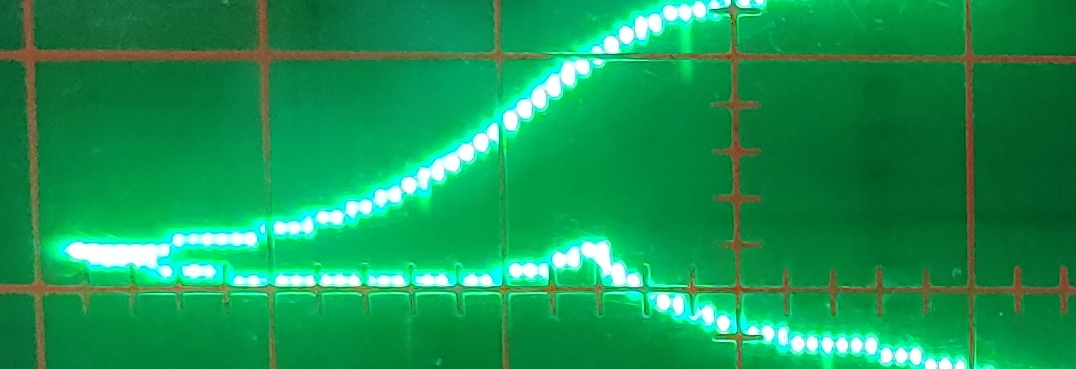
\includegraphics[width=0.99\textwidth]{images/low-resolution.png}
\caption{Low resolution leads to noticeably discrete points}
\label{fig:low-resolution}
\end{figure}

\begin{figure}[p]
\centering
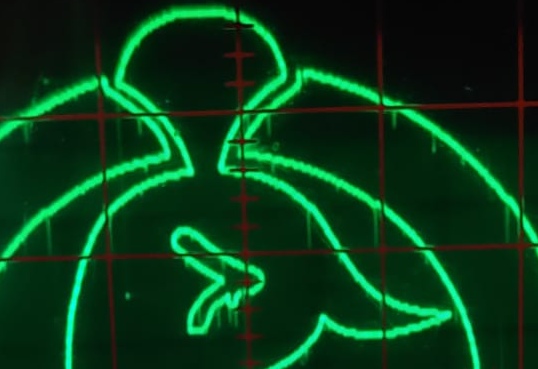
\includegraphics[width=0.49\textwidth]{images/vertical-dac-glitches1.png}\hspace{0.01\textwidth}
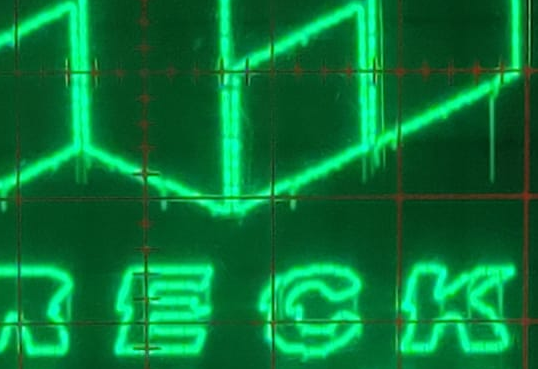
\includegraphics[width=0.49\textwidth]{images/vertical-dac-glitches2.png}
\caption{Glitches of the vertical DAC look like spikes at certain Y values}
\label{fig:vertical-dac-glitches}
\end{figure}

\begin{figure}[p]
\centering

\includegraphics[width=0.49\textwidth]{images/ringing-2d.png}\hspace{0.01\textwidth}
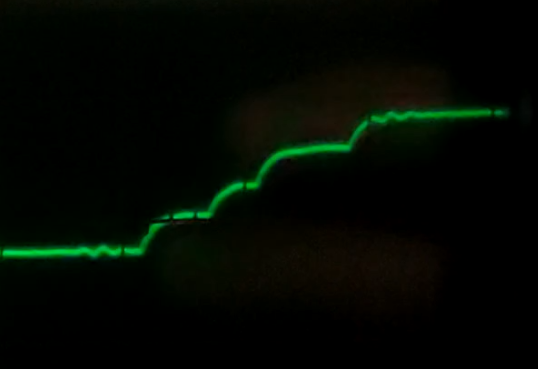
\includegraphics[width=0.49\textwidth]{images/ringing-1d.png}
\caption{Ringing and parasitic capacitance artifacts, as seen in the final image (unwanted wisps trailing off objects' corners), as well as in a Y coordinate/time graph (slow voltage transitions, unwanted oscillations).}
\label{fig:ringing}
\end{figure}

\section{Oscilloscope music, animations}

Among prior art, so called "Oscilloscope music", especially \href{https://www.youtube.com/playlist?list=PLFgoUhNvMLrr8izq38HX6rjFR-nkfklxw}{Jerobeam Fenderson's work}, stands out for its exquisite combination of graphics and sound as part of the same medium. Such works of art meticulously coordinate the two waveforms to both draw discernible shapes and animations, as well as to sound like music if interpreted as sound instead of beam coordinates.

To be able to display such works, we implement a signal streaming system, whereby the controlling computer sends uncompressed 18-bit-per-sample, 192KHz sample rate audio, and the controlled Arduino receives the data and displays it. While in principle this seems like a rather basic task, in practice it is riddled with various challenges. Ideally, we would send one sample at a time, and while the computer waits for the correct time for the next sample, the beam would stay still on the current sample, but this very inefficiently uses the USB protocol and is very slow, not allowing us to achieve 192KHz. We must group together multiple samples in so-called frames, and have the Arduino cycle through the samples of each frame in the time it takes to receive the next frame. The issue that arises is related to the fact that we cannot control the beam intensity, so when the Arduino is waiting and processing serial data, the beam will stay put for a significant period of time, accumulating to a bright spot on the screen. The longer the frames, the more time it will spend receiving and not moving the beam, leading to a tradeoff between frame lengths and image quality. (\autoref{fig:recv-alias})

Another quality enhancement we considered was using the \mbox{Arduino's} behaviour of interrupting on received data. If we send the frame in equally spaced sub-frame chunks, the "bright spots" won't only appear at frame boundaries, but also whenever the Arduino is interrupted during the actual drawing. This will have the effect of spreading out the brightness discrepancies (\autoref{fig:interrupt-hack}), but is limited, because if we split the frames too much we will arrive at the first issue of inefficiently using the USB protocol and bottlenecking the transfer rate. In the end, the results were virtually identical to reducing the frame length, so we decided the code complexity not to be worth it.

\begin{figure}[h]
\centering \def\svgwidth{0.7\linewidth} \input{interrupt-hack.pdf_tex}
\caption{Appearance of normal frames versus sub-frames.}
\label{fig:interrupt-hack}
\end{figure}

\begin{figure}[p]
\centering
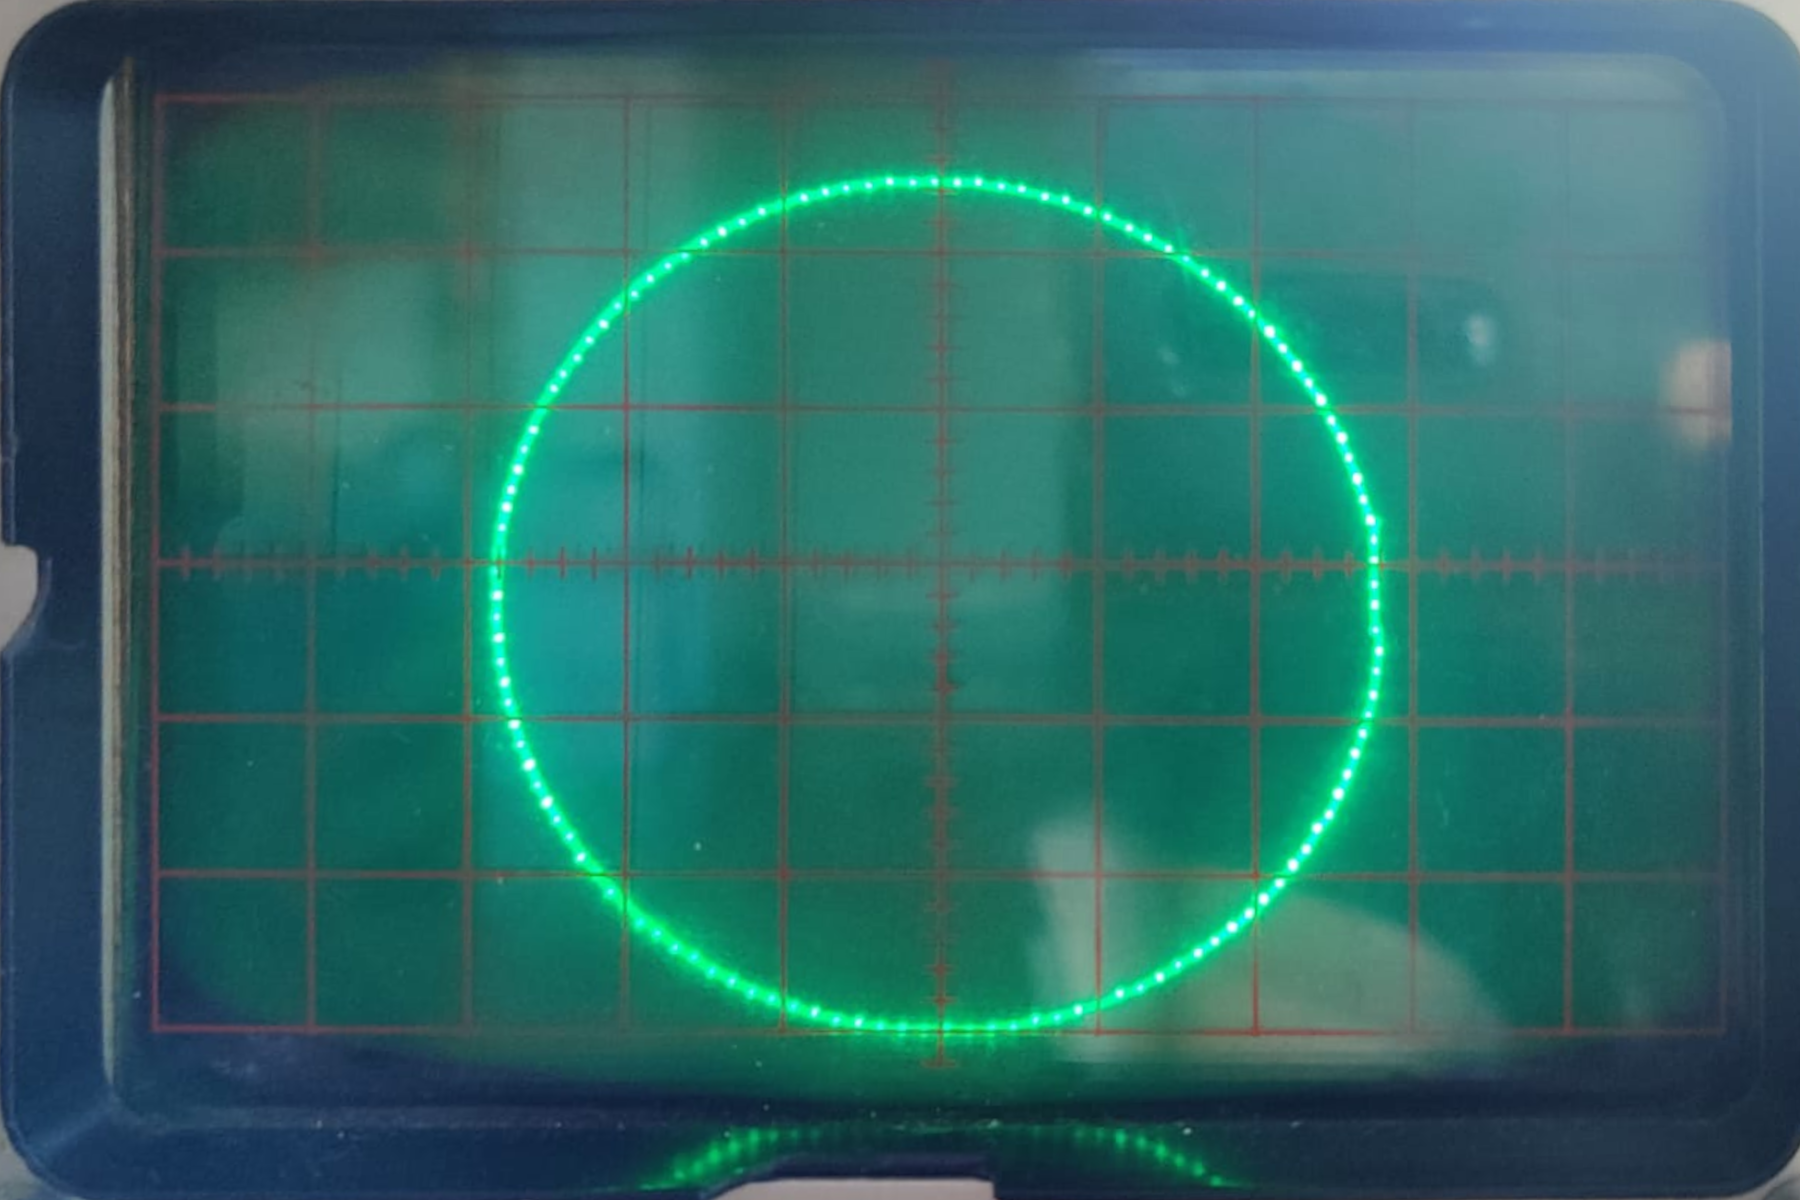
\includegraphics[width=0.49\textwidth]{images/recv-alias-16.png}\hspace{0.01\textwidth}
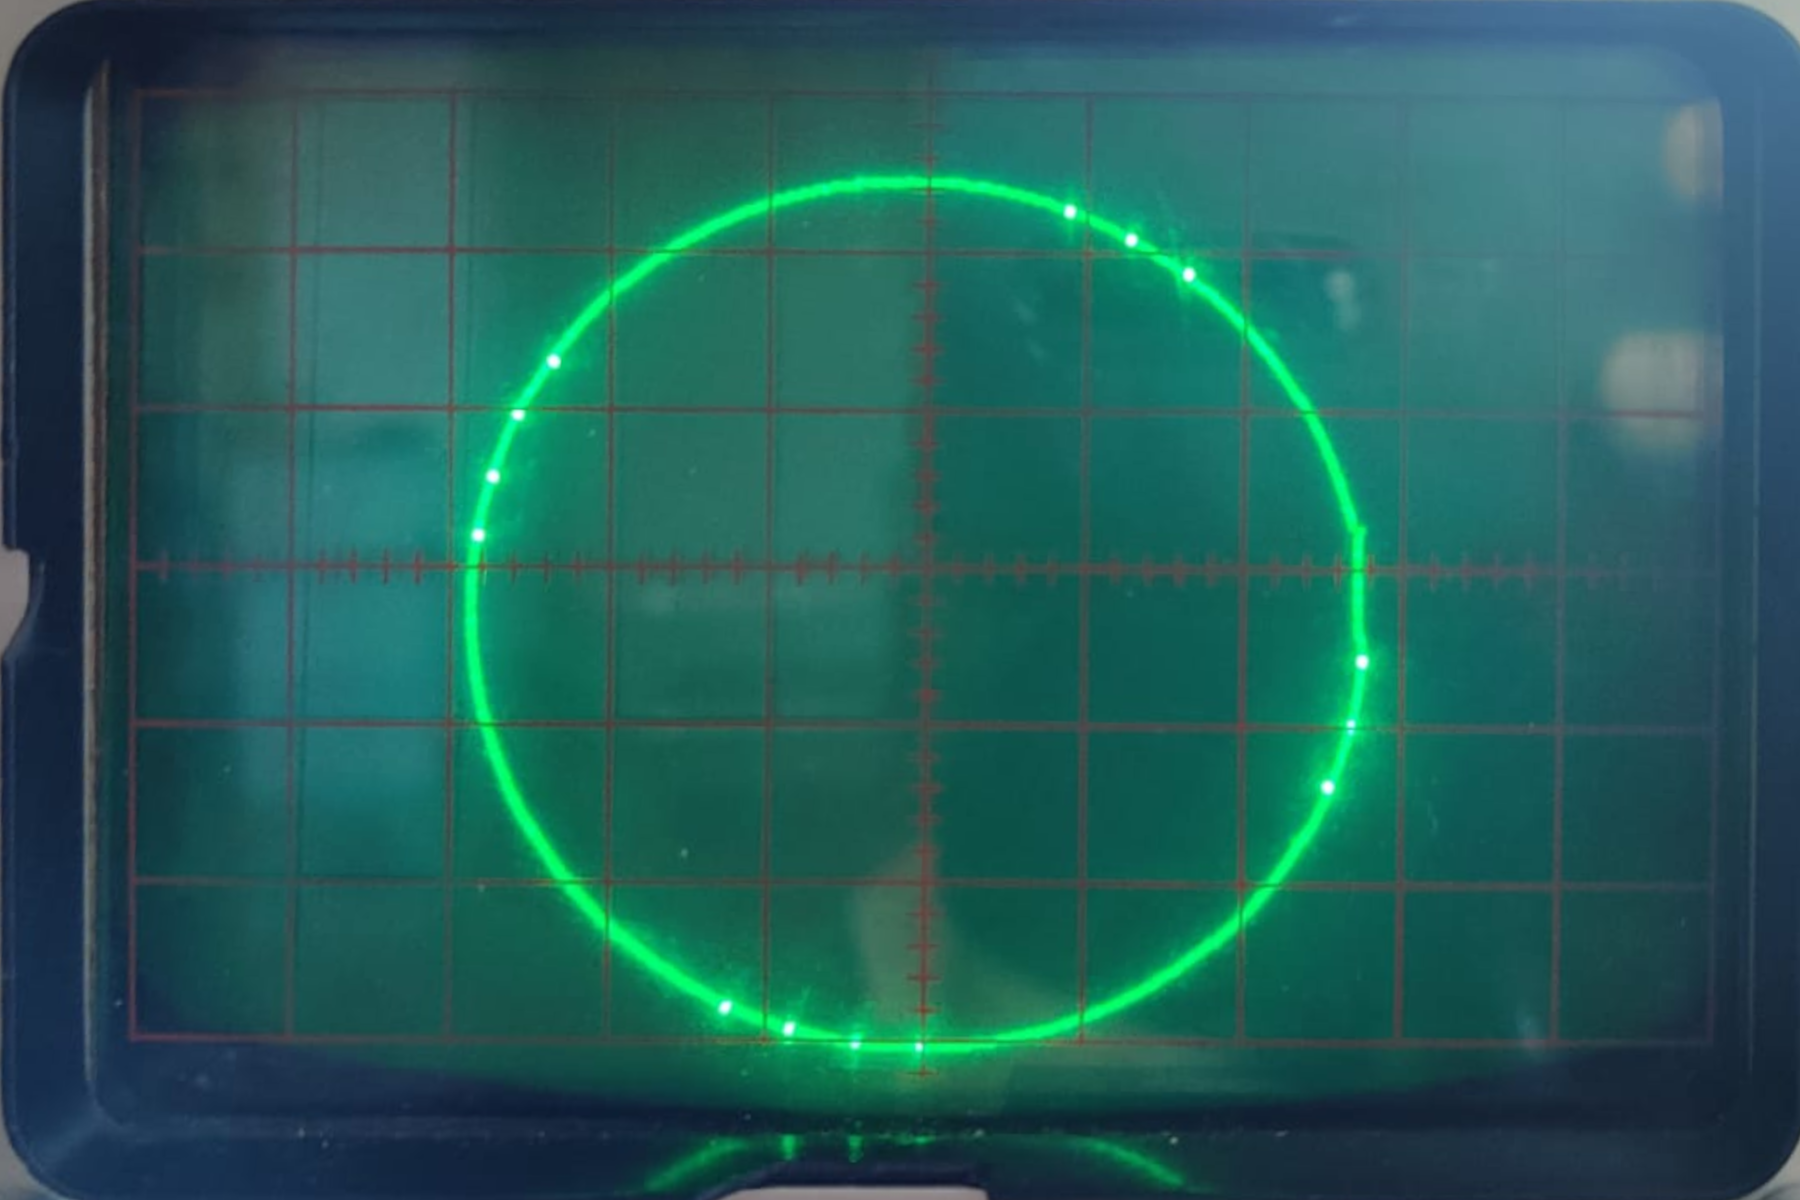
\includegraphics[width=0.49\textwidth]{images/recv-alias-256.png}\vspace{0.01\textwidth}
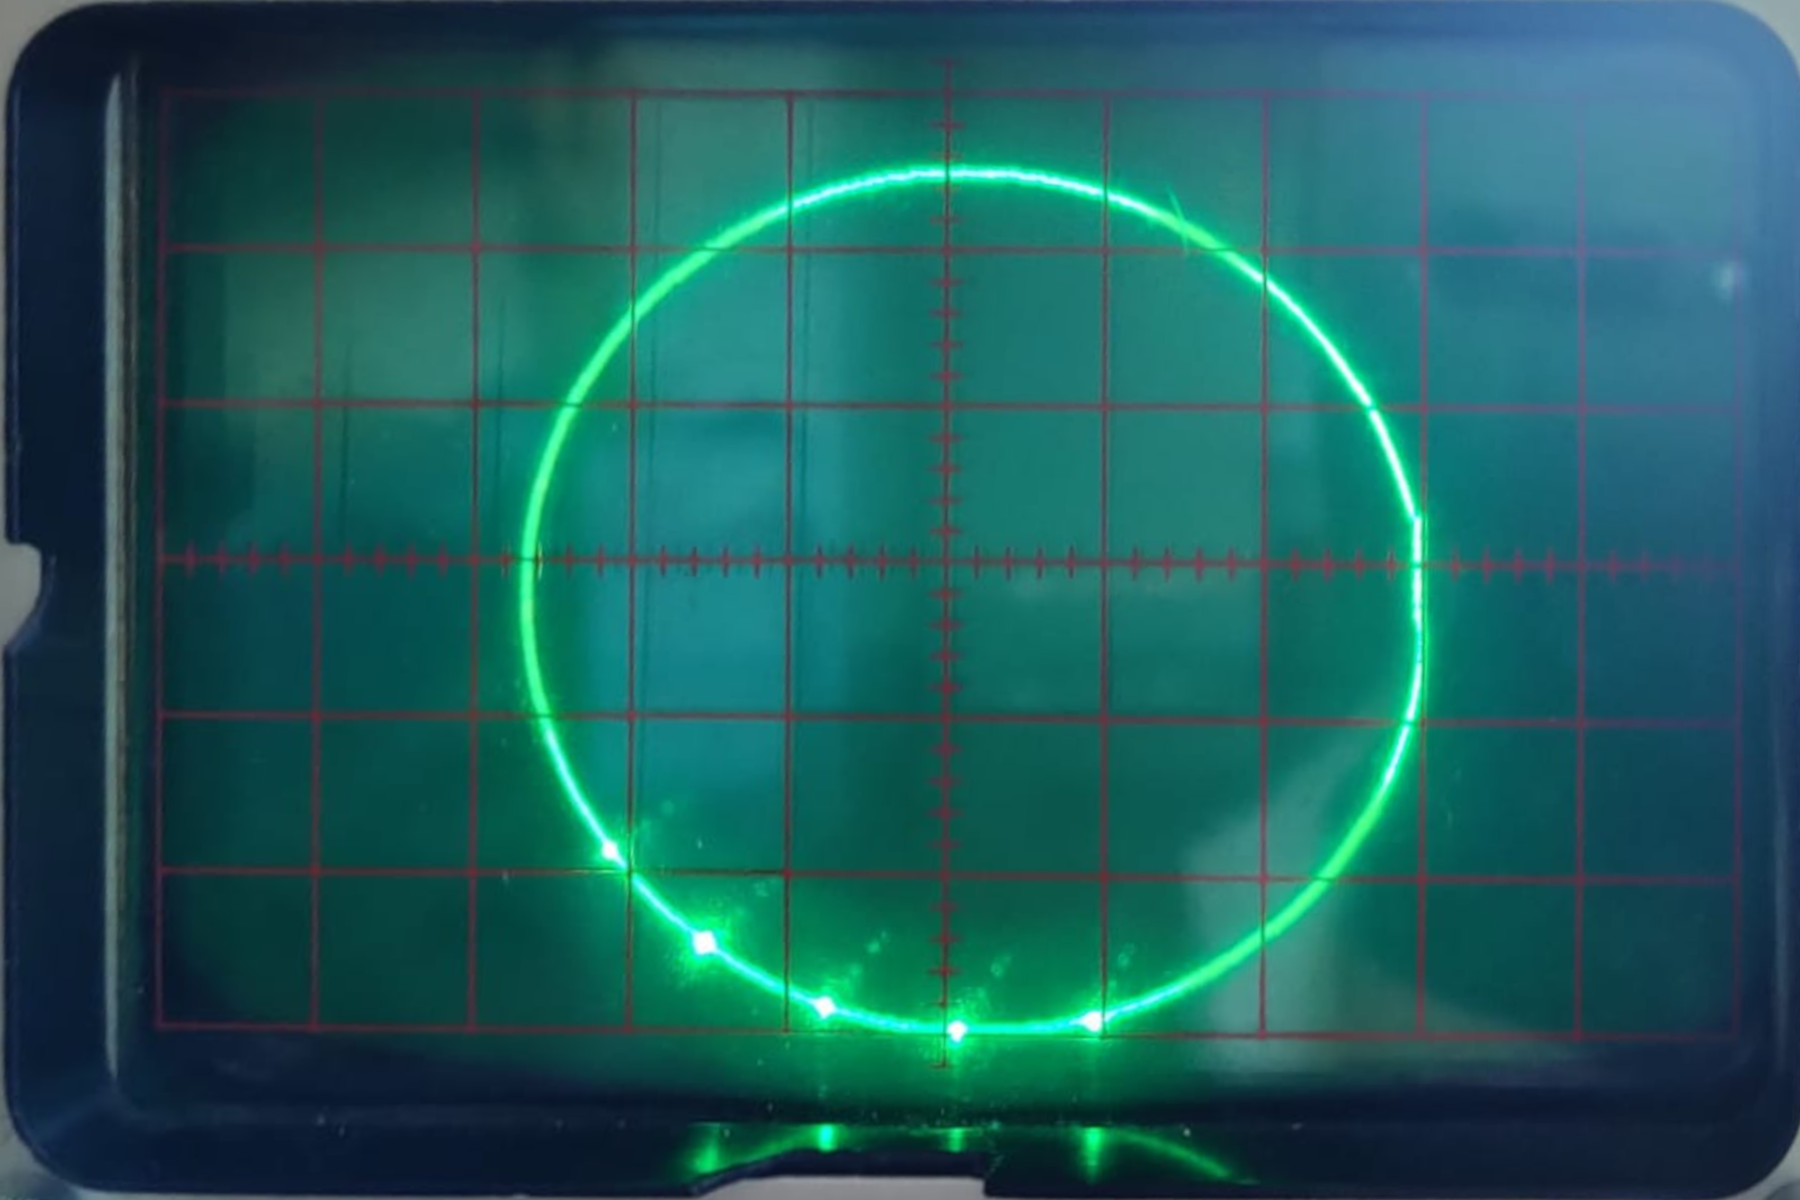
\includegraphics[width=0.49\textwidth]{images/recv-alias-2048.png}\hspace{0.01\textwidth}
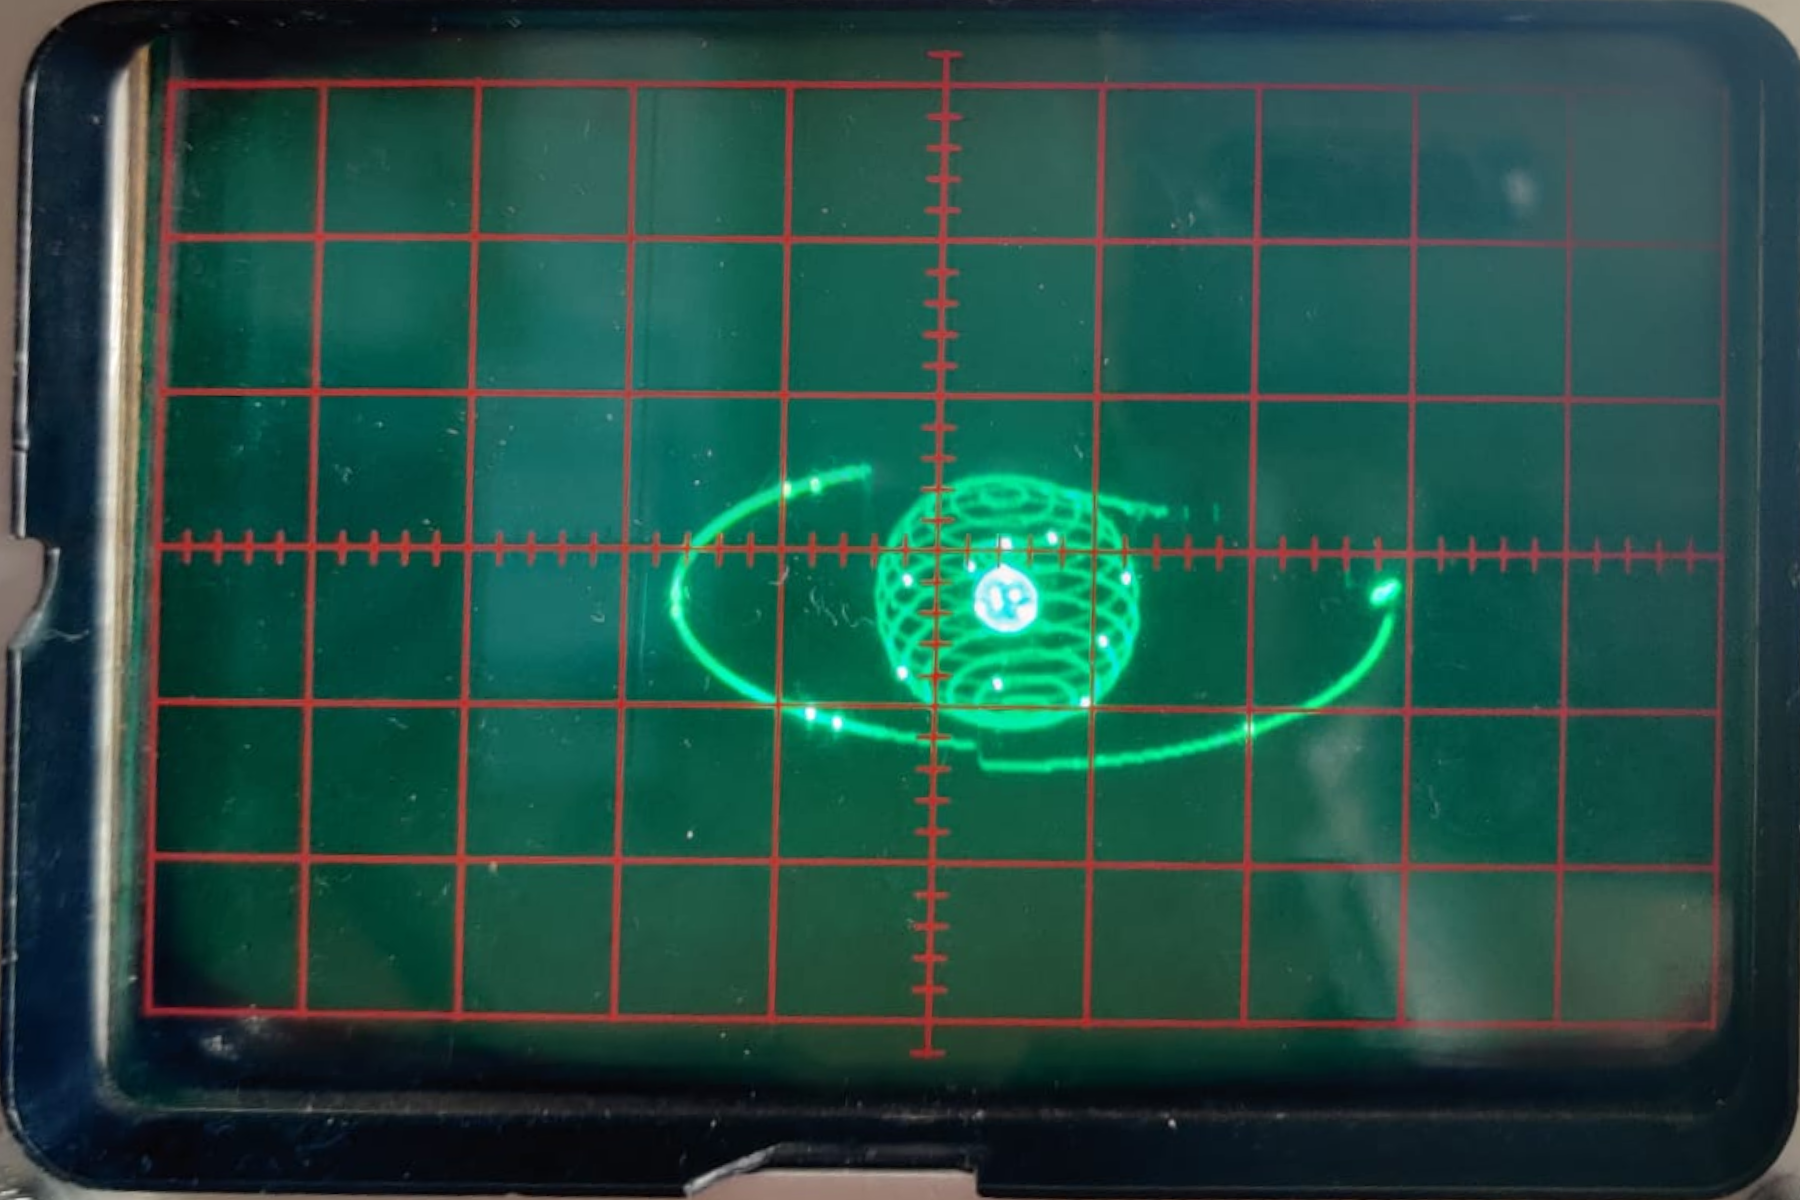
\includegraphics[width=0.49\textwidth]{images/recv-alias-anim.png}
\caption{Bright spots appear when the Arduino is idling for more sample data, or processing it. In order, 16 samples/frame, 256 samples/frame, 2048 samples/frame for a circle consisting of 1000 samples, and 192 samples/frame during an arbitrary animation.}
\label{fig:recv-alias}
\end{figure}

\section{Static and animated demonstration}

For the complete proof of concept, we combine the two functionalities presented in the previous sections in a single system. The Arduino shall start up displaying a fixed "splash screen", and repeatedly attempt a handshake over serial with a compatible controller program, following a very simple communication protocol.

\begin{multicols}{2}

\noindent Controller handshake

\begin{lstlisting}
serial.recvuntil(b"Hello?\r\n")
serial.send(b"!")
serial.recvuntil("Hello!\r\n")
N = int(serial.recvline()
        .decode().strip())
\end{lstlisting}

\columnbreak

\noindent Arduino handshake

\begin{lstlisting}
long last = millis();
do {
  // draw logo
  for (int i = 0; i < num; i++) {
    point(logo[i].x, logo[i].y);
  }
  
  // try handshake every 500ms
  long now = millis();
  if (now - last > 500) {
    Serial.println("Hello?");
    last = now;
  }
} while (Serial.read() != '!');
Serial.println("Hello!");
Serial.println(N);
\end{lstlisting}

\end{multicols}

During the handshake, the Arduino communicates the length of its point buffer (i.e., the frame length), which is used by the controlling program to split the path into correctly sized frames. A stereo wav file is used as a source for the path animation data. The controller parses the wav file in chunks, converts the 16 bit data to values in the expected DAC range, and re-packs the values in a binary format understood by the Arduino:

\begin{lstlisting}
for _ in range(wav.getnframes() // n):
    wav_data = wav.readframes(n)
    
    # map values to [0, 1]
    samples = [(a / 65536 + 0.5, b / 65536 + 0.5)
        for a, b in struct.iter_unpack("hh", wav_data)]
    assert all(0 <= a <= 1 and 0 <= b <= 1 for a, b in samples)

	# repack remapped data to {uint16_t X; uint8_t Y;} 
    serial.send(b''.join(
        struct.pack("<HB", int(a*728), int(b*255))
        for a,b in samples
    ))
\end{lstlisting}

The Arduino fills up a fixed size buffer with data from the serial interface, and then draws the points in a loop:

\begin{lstlisting}
unsigned int recvd = 0, rem = sizeof(buf);
while (rem > 0) {
  const auto count = Serial.readBytes((char*) buf + recvd, rem);
  recvd += count;
  rem -= count;
}
for (int i = 0; i < N; i++) {
  point(buf[i].x, buf[i].y);
}
\end{lstlisting}

The device starts by displaying the TUCN logo as seen in \autoref{fig:tucn-full}. When the controller software is started, the Arduino switches to the live streamed points, as seen in the following images. (Jerobeam Fenderson -- Planets, Blocks, Shrooms, Reconstruct) \href{https://youtu.be/MOuCXOf-fcU}{A full demonstration can be found on Youtube}.

\begin{figure}[h]
\centering
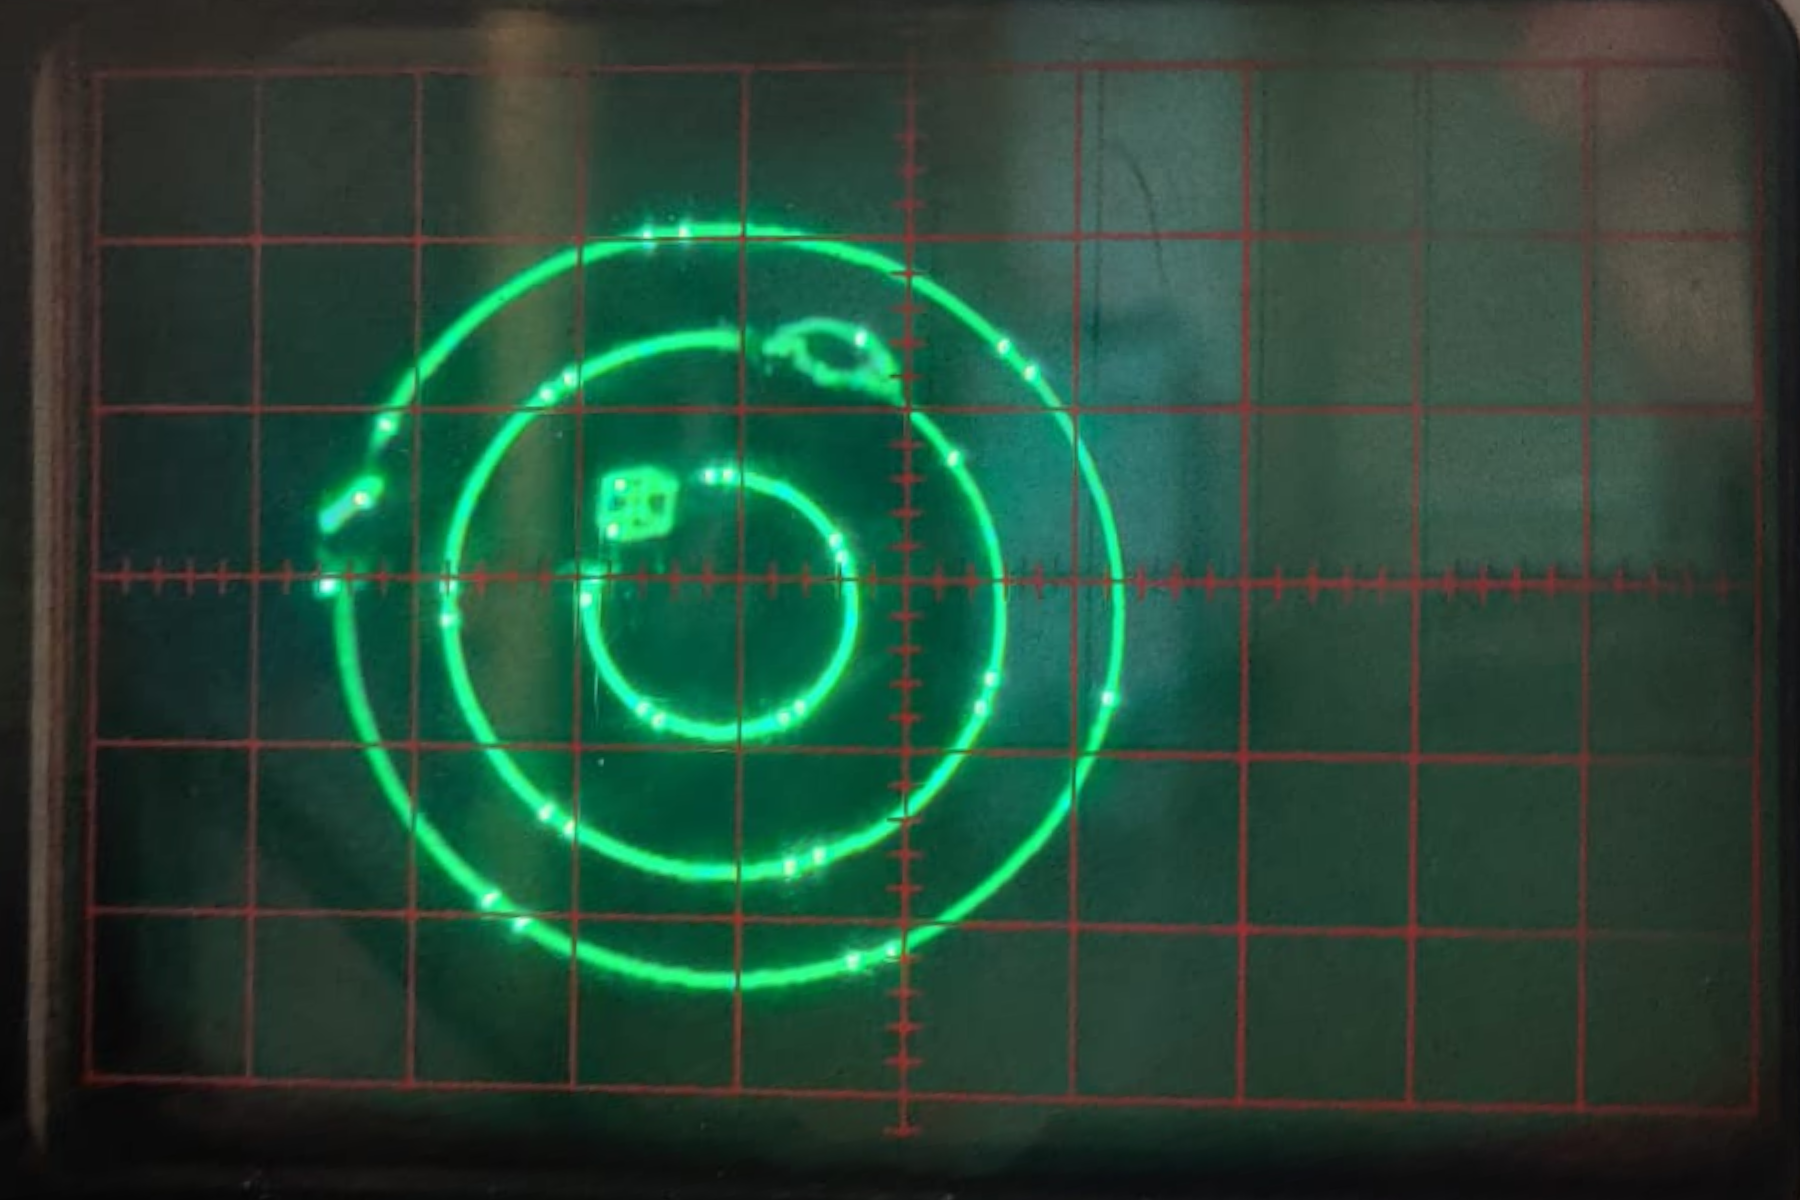
\includegraphics[width=0.49\textwidth]{images/demo1.png}\hspace{0.01\textwidth}
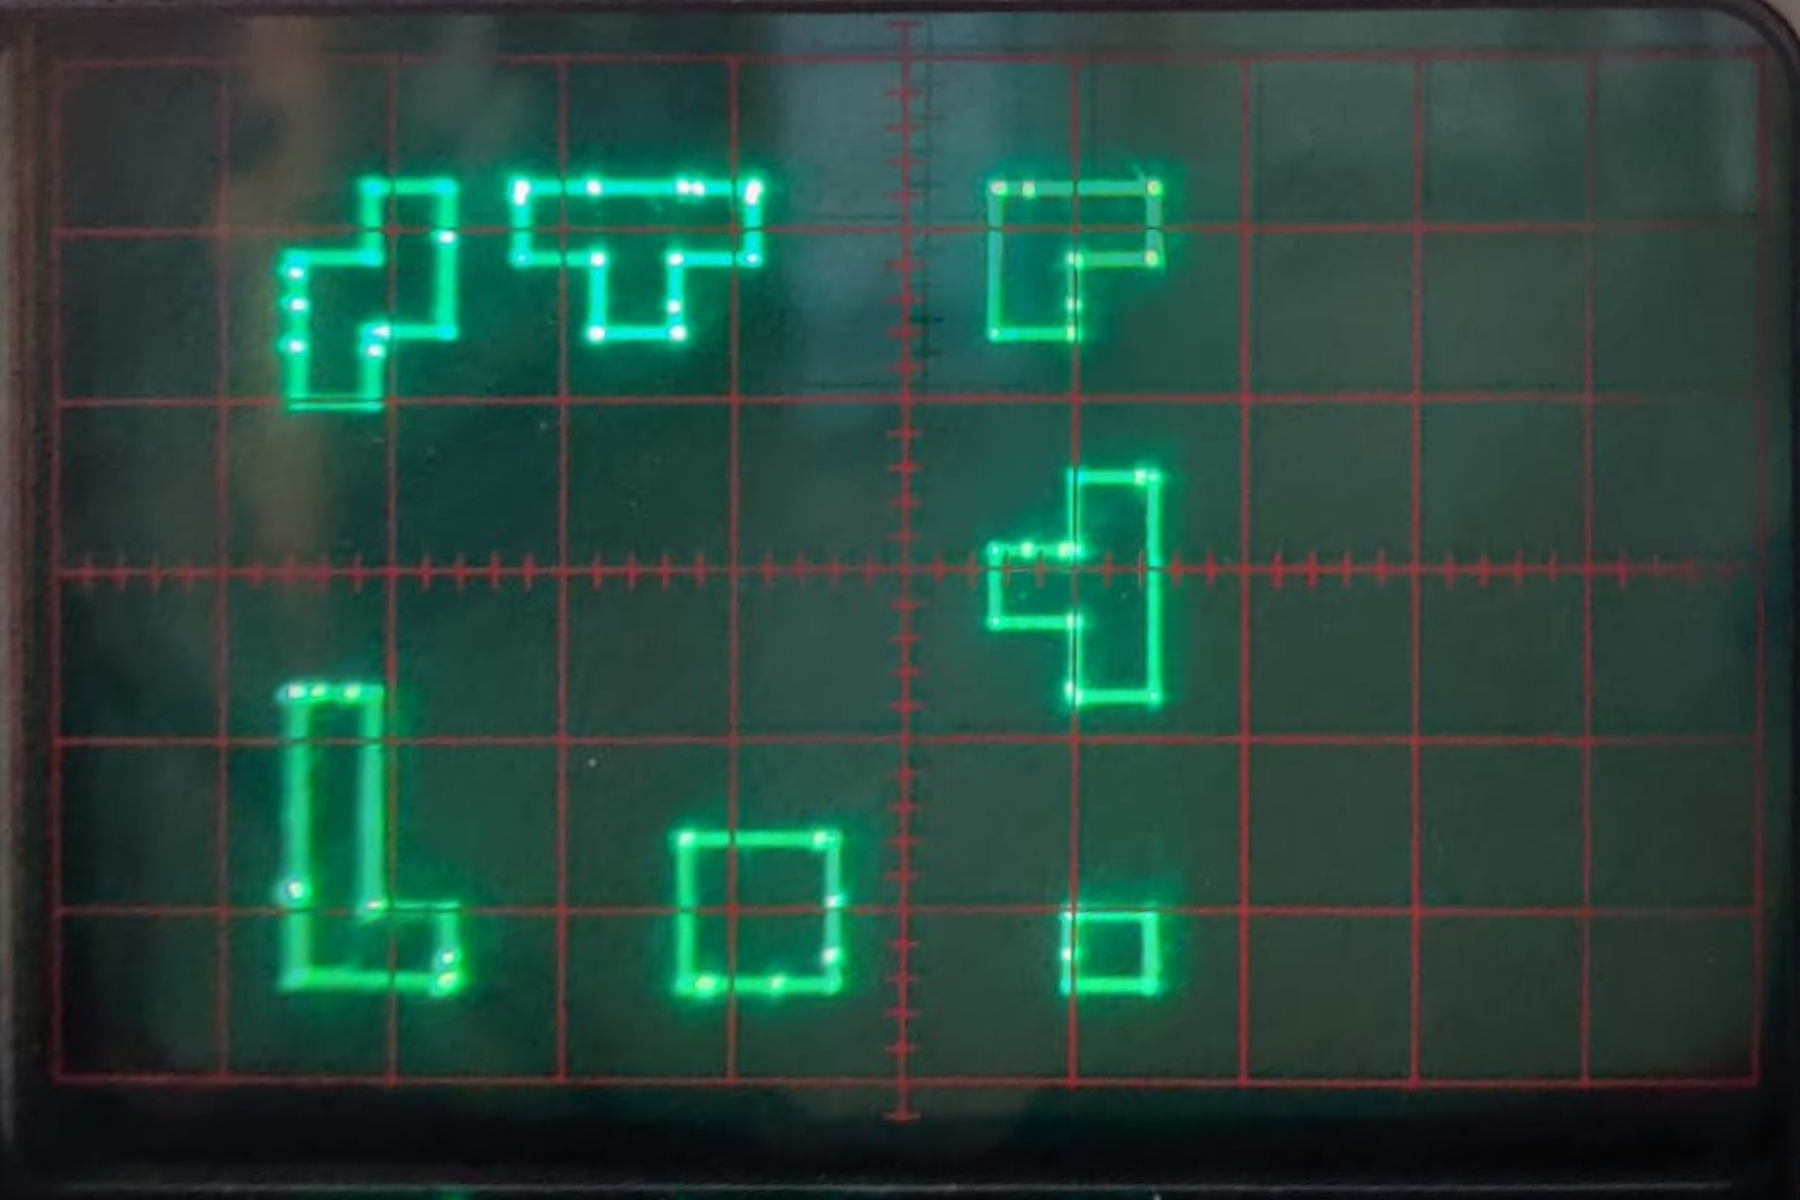
\includegraphics[width=0.49\textwidth]{images/demo2.png}\vspace{0.01\textwidth}
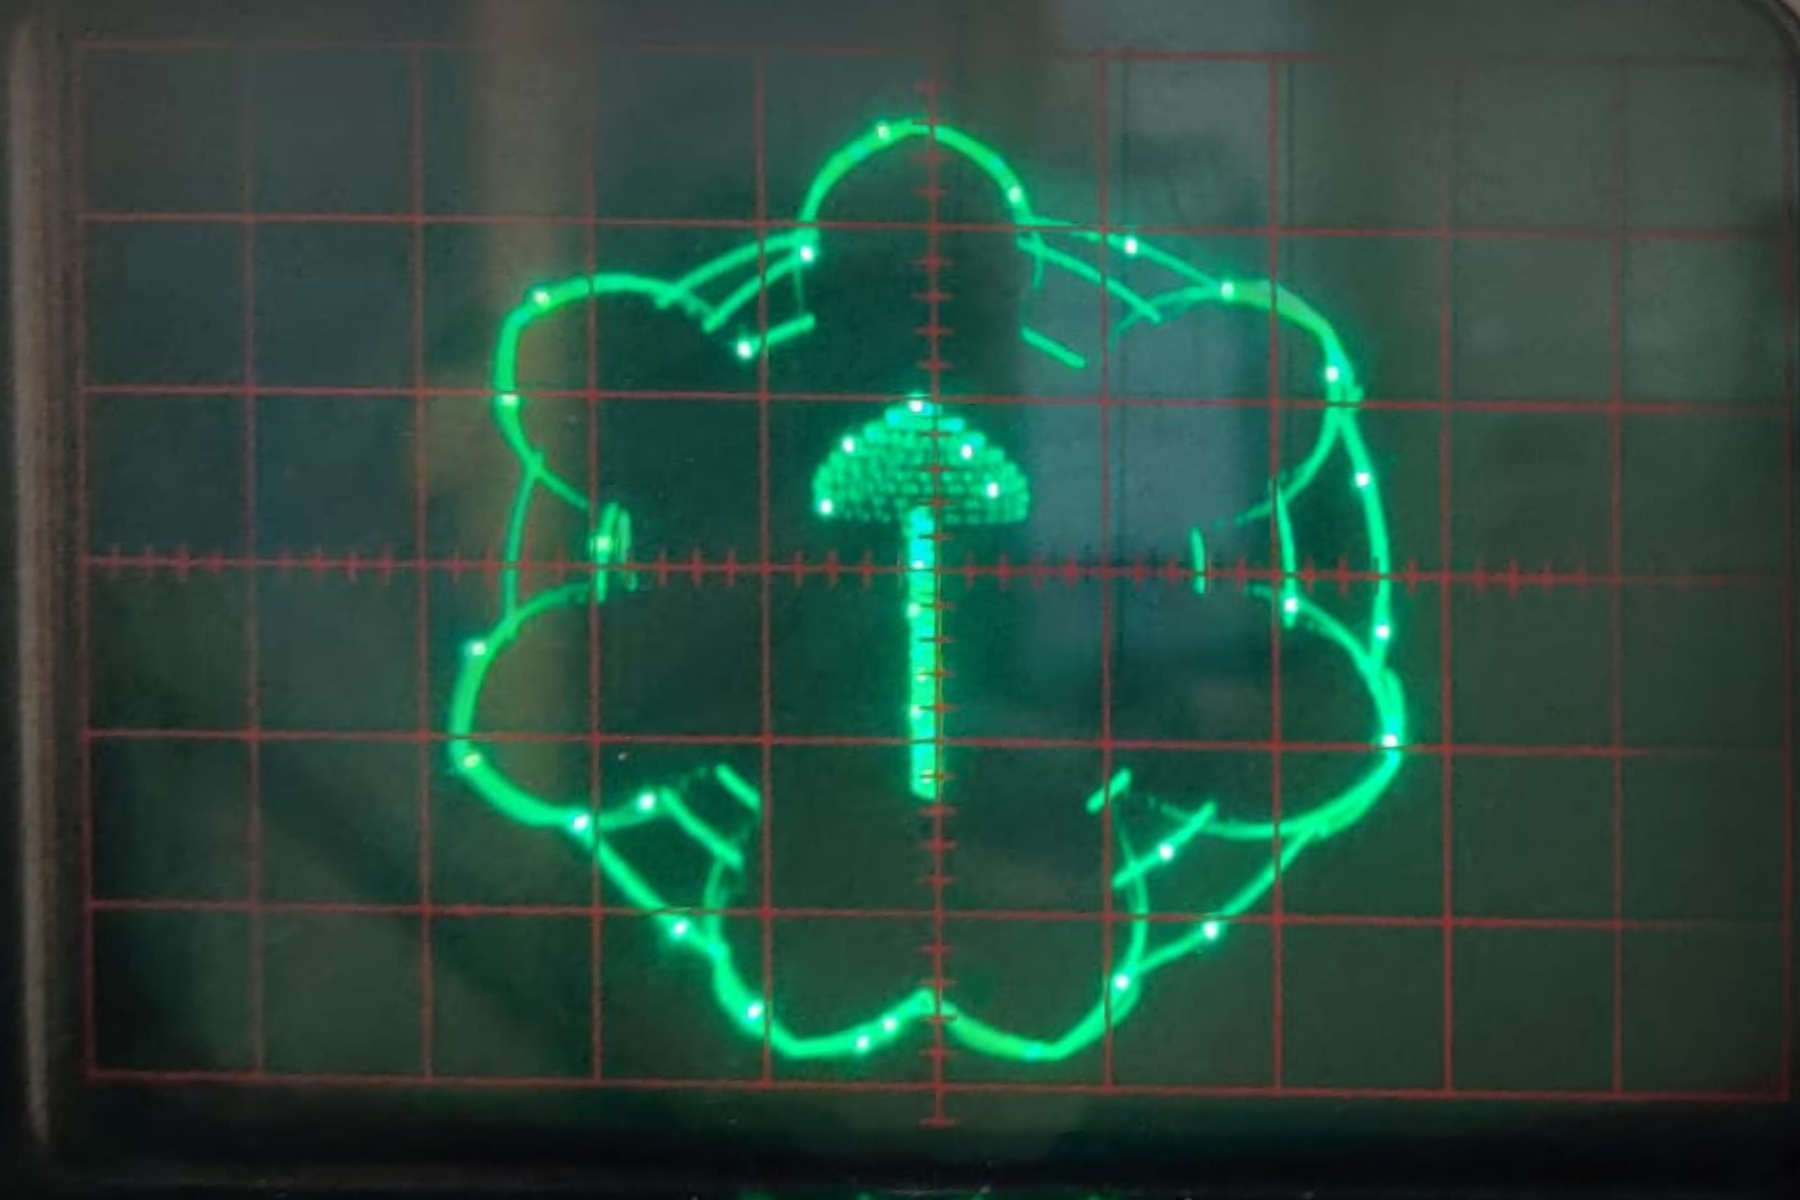
\includegraphics[width=0.49\textwidth]{images/demo3.png}\hspace{0.01\textwidth}
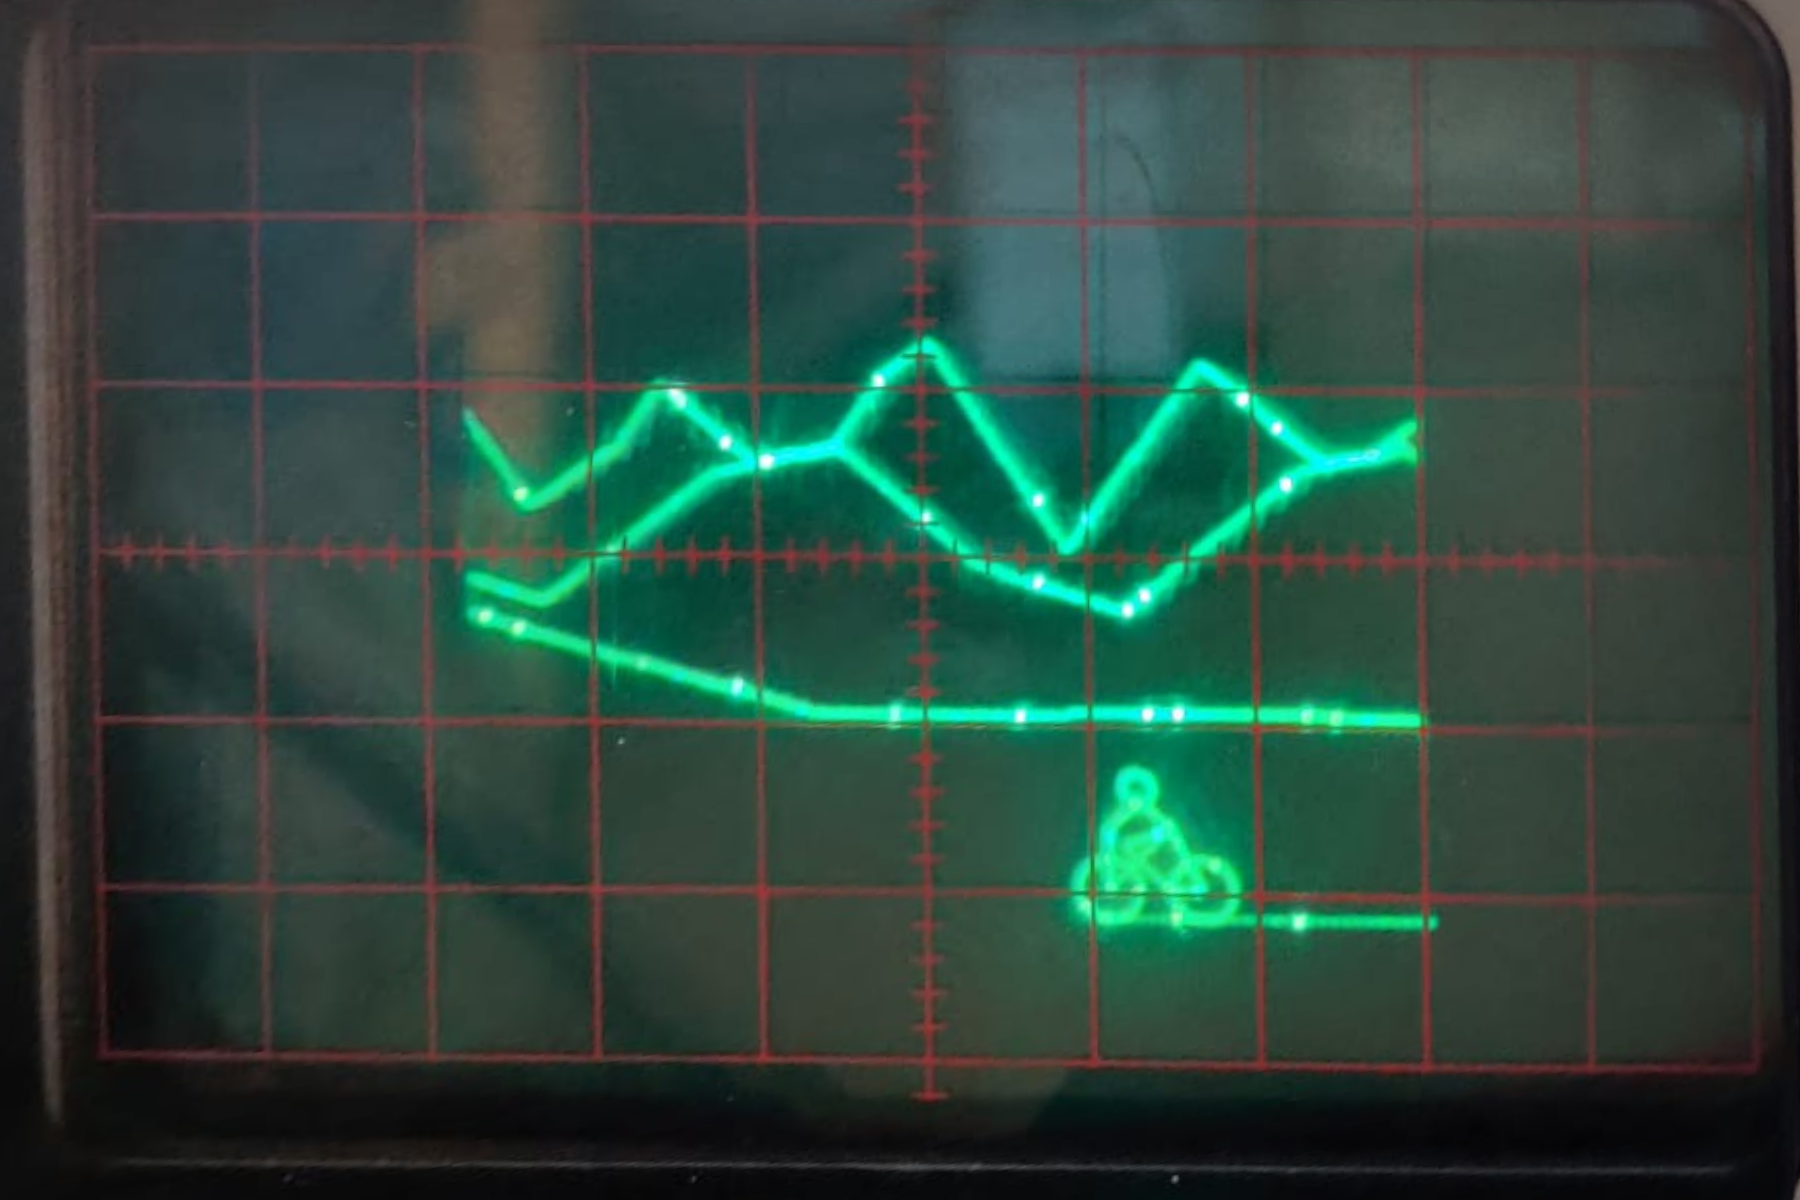
\includegraphics[width=0.49\textwidth]{images/demo4.png}
\end{figure}

\newpage
\begin{appendices}
\section{SVG path to C header conversion}
\label{appendix:svg2header}
\href{https://github.com/trupples/oscilloscope-graphics/blob/main/convert-svg-to-header.js}{This code is available on github.}
\lstinputlisting{convert-svg-to-header.js}

\newpage
\section{Basic signal generation}
\label{appendix:staticvector}
\href{https://github.com/trupples/oscilloscope-graphics/blob/main/static-vector/static-vector.ino}{This code is available on github.}
\lstinputlisting{static-vector/static-vector.ino}

\newpage
\section{Dissasembly comparison of bitmap calculation versus lookup}
\label{appendix:lutoptimisation}

\begin{multicols}{2}

\noindent Computing bit pattern online:
\begin{lstlisting}
MOVS    R0, #0x80
LDRB    R2, [R7,#2]
LSLS    R0, R0, #0xC
LSLS    R3, Y, #0x14
LSLS    R1, Y, #0xE
ANDS    R1, R5
ANDS    R3, R6
ORRS    R3, R1
LSLS    R1, Y, #0xF
ANDS    R1, R0
MOVS    R0, #0xC0
ORRS    R3, R1
LSLS    R0, R0, #2
LSLS    R1, Y, #3
ANDS    R1, R0
ORRS    R3, R1
MOVS    R1, #0x80
LSLS    Y, Y, #4
LSLS    R1, R1, #4
ANDS    R2, R1
ORRS    R3, R2
LDR     R2, =0x41004400
STR     R3, [R2,#0x10]
\end{lstlisting}

\columnbreak
\noindent Using a lookup table of precomputed bit patterns:

\begin{lstlisting}
LDR     R3, =porta_bitmap_lut
LSLS    R5, R5, #2
LDR     R2, [R5,R3]
LDR     R3, =0x41004400
STR     R2, [R3,#0x10]
\end{lstlisting}

\end{multicols}

\end{appendices}
\end{document}
